\newpage
\section{Versuchsaufbau}

    \subsection{Szenario}

    Im ersten Schritt wurde das Netzwerk mithilfe von Subnetting getrennt und anschließend unter Verwendung von managebaren NETGEAR-Switches
    in unterschiedliche VLANs unterteilt.

    \subsection{Durchführung}

        \subsubsection{Funktionsprüfung des Netzwerks}
        \begin{table}[H]
            \centering
            \begin{tabular}{l|c|l|c|l|c|l|c|l|c|}
            \multicolumn{1}{l}{} & \multicolumn{1}{l}{PC1} & \multicolumn{1}{l}{PC2} & \multicolumn{1}{l}{PC3} & \multicolumn{1}{l}{PC4}  \\ 
            \cline{2-5}
            PC1&&X&& \\ 
            \cline{2-5}
            PC2&X&&& \\
            \cline{2-5}
            PC3&&&&X \\
            \cline{2-5}
            PC4&&&X& \\
            \cline{2-5}
            \end{tabular}
            \caption{Ergebnistabelle\\ (Erreichbarkeit der einzelnen PCs untereinander) mittels "`ping"'-command}
        \end{table}
        
        \subsubsection{Unterteilung in Subnetze}
        Im folgenden Screenshot ist unser Netzwerkplan dokumentiert, welcher als Grundlage für
        den Versuchsaufbau fungiert.
        \begin{figure}[H]
            \centering
            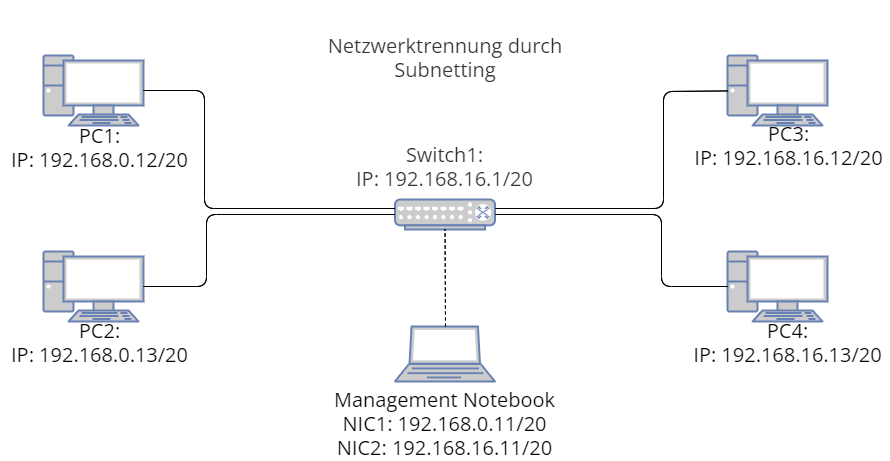
\includegraphics[scale=0.5]{images/Unterteilung in Subnetze/Netzwerkplan_Subnetting_new.png}
            \caption{Netzwerkplan Subnetting}
        \end{figure}
        Die beiden folgenden Screenshots zeigen, dass im Netzwerk zwei PCs erreichbar sind. Im ersten Netzwerk (192.168.0.0) 
        sind die Clients 1 und 2 mit den IP-Adressen 192.168.0.12 und 192.168.0.13 zu finden, während sich im zweiten Netzwerk 
        (192.168.16.0) die Clients 3 und 4 mit den IP-Adressen 192.168.16.12 und 192.168.16.13 befinden. Der Switch(192.168.16.1)
        befindet sich im zeiten Netzwerk(192.168.16.0).
        \begin{figure}[H]
        \centering
            \begin{subfigure}{.5\textwidth}
              \centering
              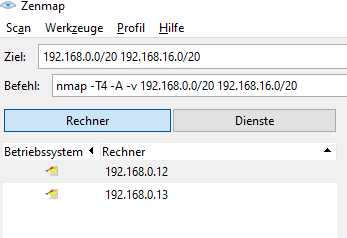
\includegraphics[scale=0.7]{images/Unterteilung in Subnetze/Scan_Subnetz_1.png}
              \caption{Subnetz 1 (192.168.0.0)}
            \end{subfigure}%
            \begin{subfigure}{.5\textwidth}
              \centering
              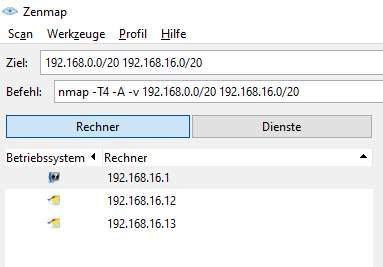
\includegraphics[scale=0.7]{images/Unterteilung in Subnetze/Scan_Subnetz_2.png}
              \caption{Subnetz 2 (192.168.16.0) mit Switch}
            \end{subfigure}
        \caption{Zenmap-Scan Subnetze}
        \end{figure}
        
        Es ist ersichtlich, dass die Clients der beiden Netzwerke nicht miteinander kommunizieren können, wodurch eine abteilungsübergreifende 
        Erreichbarkeit der PCs nicht mehr möglich ist. Dies ist auch in den beiden folgenden Screenshots deutlich erkennbar, 
        in denen der Befehl "`ipconfig"' und "`ping"' in der Befehlszeile des jeweiligen Clients ausgeführt wurde.
        
        \begin{figure}[H]
        \centering
            \begin{subfigure}{\textwidth}
                \centering
                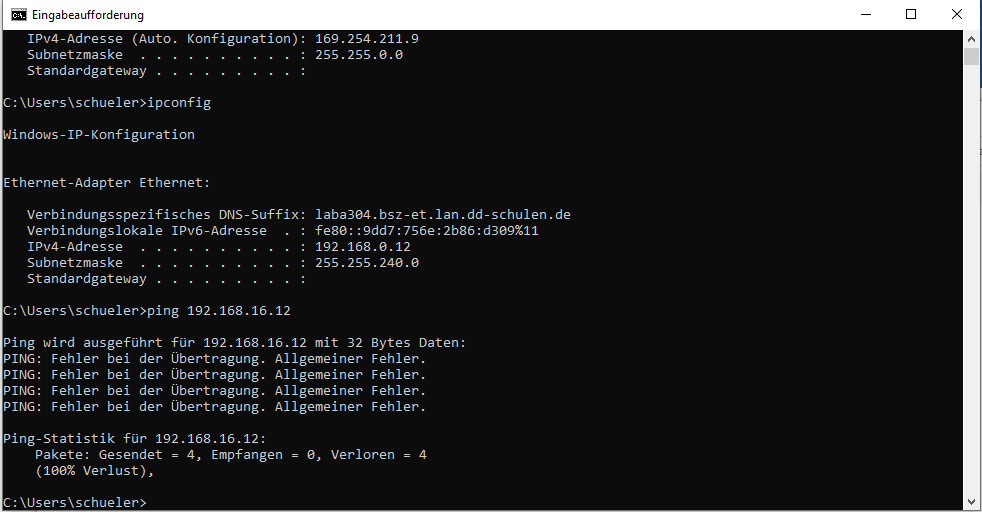
\includegraphics[scale=0.5]{images/Unterteilung in Subnetze/SubnetzPC1_PingPC3.png}
                \caption{ping PC1 zu PC3}
            \end{subfigure}
            \begin{subfigure}{\textwidth}
                \centering
                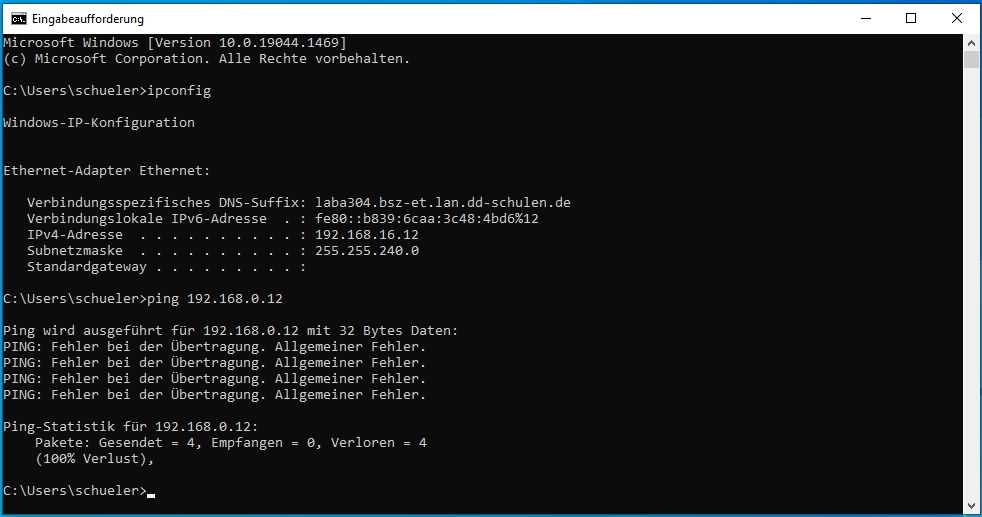
\includegraphics[scale=0.5]{images/Unterteilung in Subnetze/SubnetzPC3_PingPC1.png}
                \caption{ping PC3 zu PC1}
            \end{subfigure}
        \caption{Erreichbarkeit Netzwerke Subnetting}
        \end{figure}

        \newpage
        \subsubsection{Trennung durch VLAN herstellen}
        Im folgenden Screenshot ist unser Netzwerkplan dokumentiert, welcher als Grundlage für
        den Versuchsaufbau der Netzwertrennung durch VLANs fungiert. Dieser Netzwerkplan wird auch
        in den nächsten 2 Abschnitten genutzt.
        \begin{figure}[H]
            \centering
            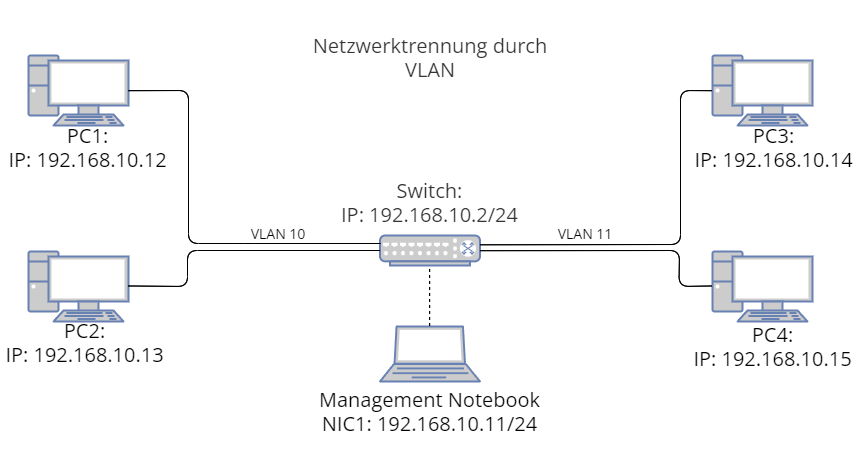
\includegraphics[width=\linewidth]{images/Trennung durch VLAN herstellen/Netzwerkplan_VLAN._portbasiert.png}
            \caption{Netzwerkplan portbasiertes VLAN}
        \end{figure}
        Um die Trennung durch VLANs zu realisieren haben wir als erstes ein portbasiertes VLAN eingerichtet, welches wir
        anschließend auf PVID erweitert haben.
        \begin{figure}[H]
        \centering
            \begin{subfigure}{\linewidth}
                \centering
                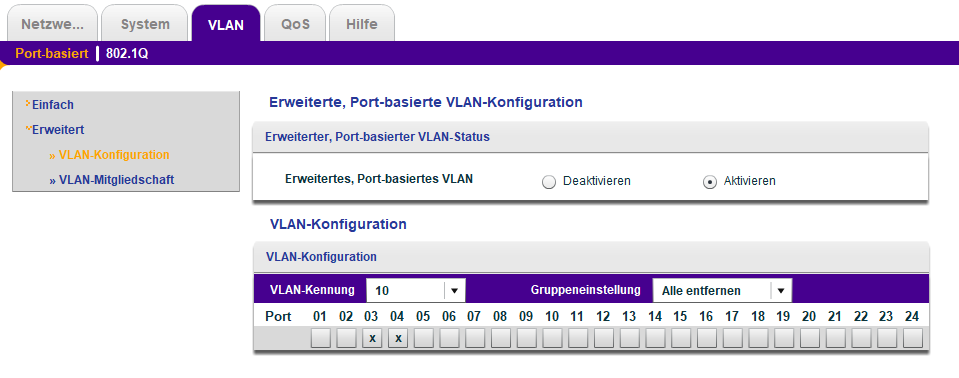
\includegraphics[scale=0.45]{images/Trennung durch VLAN herstellen/VLAN10_Konfiguration.png}
                \caption{VLAN10 Konfiguration}
            \end{subfigure}
            \begin{subfigure}{\linewidth}
                \centering
                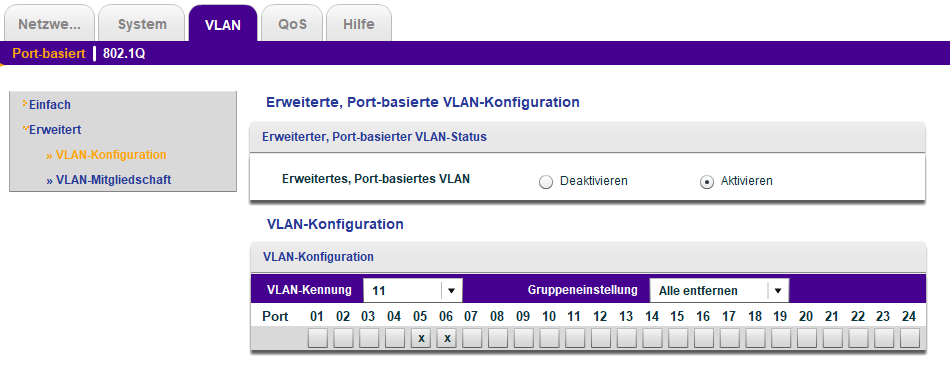
\includegraphics[scale=0.45]{images/Trennung durch VLAN herstellen/VLAN11_Konfiguration.png}
                \caption{VLAN11 Konfiguration}
            \end{subfigure}
        \caption{Konfiguration des portbasierten VLANs}
        \end{figure}

        \newpage
        Die Clients sind hierbei in zwei VLANs getrennt, 10 und 11. In den folgenden Screenshots sind Erreichbarkeiten
        der anderen Clients an dem jeweiligen Client dokumentiert.
        \begin{figure}[H]
        \centering
            \begin{subfigure}{.45\linewidth}
                \centering
                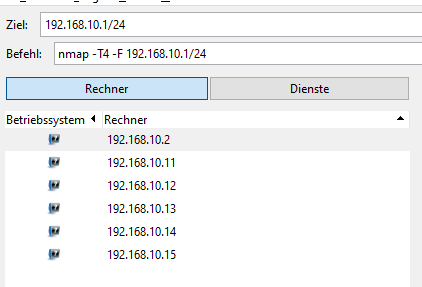
\includegraphics[width=\linewidth]{images/Trennung durch VLAN herstellen/ErreichbarkeitAnliegendAn11.png}
                \caption{Erreichbarkeit anliegend an Management Notebook}
            \end{subfigure}
            \begin{subfigure}{.45\linewidth}
                \centering
                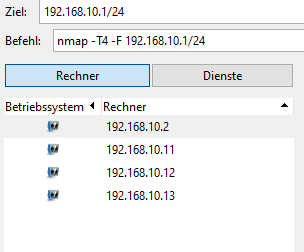
\includegraphics[width=\linewidth]{images/Trennung durch VLAN herstellen/ErreichbarkeitAnliegendAn12.png}
                \caption{Erreichbarkeit anliegend an PC1}
            \end{subfigure}
            \begin{subfigure}{\textwidth}
                \centering
                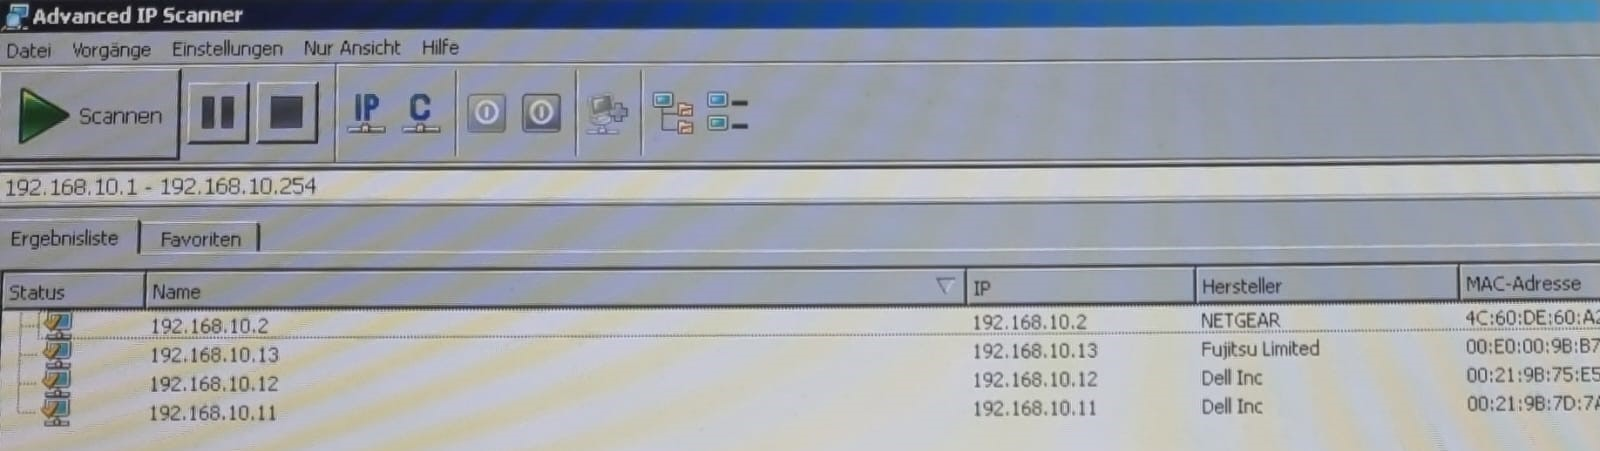
\includegraphics[width=\linewidth]{images/Trennung durch VLAN herstellen/ErreichbarkeitAnliegendAn13.jpg}
                \caption{Erreichbarkeit anliegend an PC2}
            \end{subfigure}
            \begin{subfigure}{\textwidth}
                \centering
                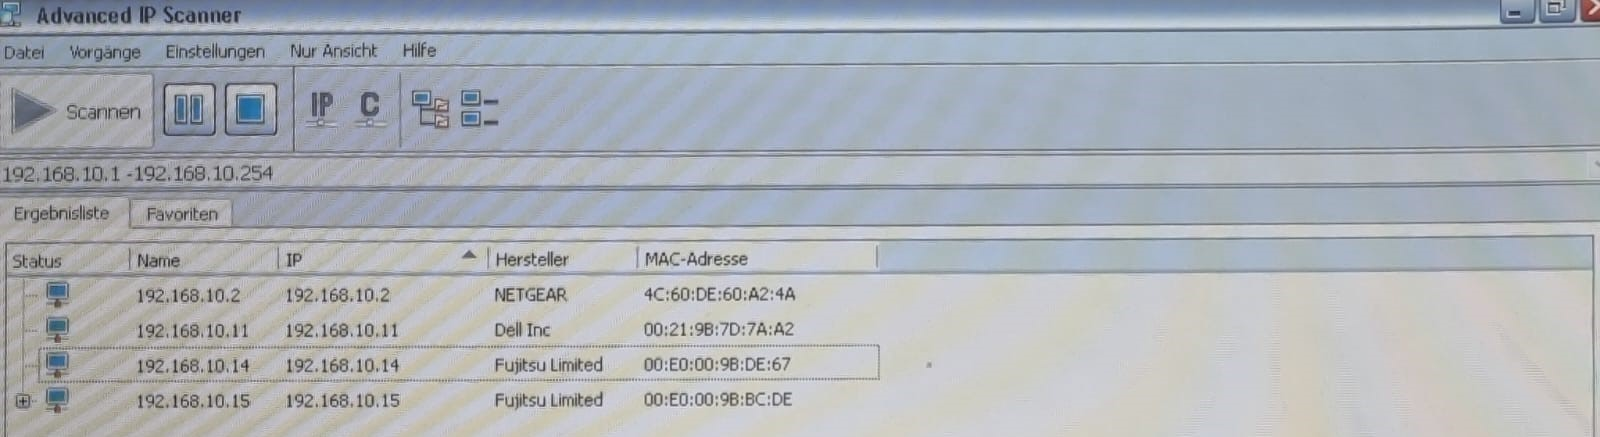
\includegraphics[width=\linewidth]{images/Trennung durch VLAN herstellen/ErreichbarkeitAnliegendAn14.jpg}
                \caption{Erreichbarkeit anliegend an PC3}
            \end{subfigure}
            \begin{subfigure}{\textwidth}
                \centering
                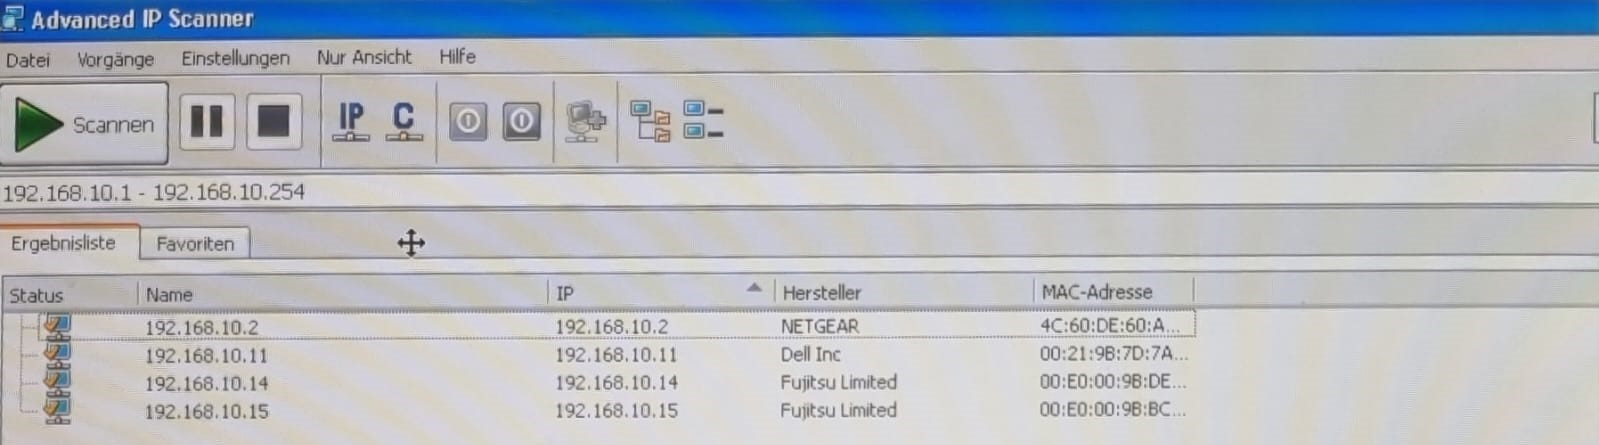
\includegraphics[width=\linewidth]{images/Trennung durch VLAN herstellen/ErreichbarkeitAnliegendAn15.jpg}
                \caption{Erreichbarkeit anliegend an PC4}
            \end{subfigure}
        \caption{Erreichbarkeiten im portbasierten VLAN}
        \end{figure}
        Aus den oben aufgezeigten Screenshots lässt sich erkennen, dass ausschließlich die Clients der 
        zugehörigen VLANs miteinander kommunizieren können.


        \newpage
        \subsubsection{VLAN übergreifenden Server integrieren}

        \newpage
        \subsubsection{Einrichtung Layer2-Switche}